\documentclass[11pt]{article}
\usepackage[english]{babel}
\usepackage[utf8]{inputenc}
\usepackage{amsmath}
\usepackage{graphicx}
\usepackage[colorinlistoftodos]{todonotes}
\usepackage{enumitem}
\usepackage{listings}
\usepackage{filecontents}
\usepackage{verbatim}
\usepackage{eurosym}
\usepackage[export]{adjustbox}
\usepackage[T1]{fontenc}
\usepackage{subfig}
\usepackage[backend=biber, style=apa, sorting=ynt]{biblatex}
\setlength\bibitemsep{1.9\itemsep}
\addbibresource{ref.bib}
\usepackage{float}
\usepackage[a4paper,top=2.5cm,bottom=2cm,left=2cm,right=2cm,marginparwidth=1.75cm]{geometry}
\usepackage{tabularx, multirow, makecell, booktabs, caption, subcaption}
\usepackage{tikz,,color,fullpage,,epsf}
\usepackage{array}
\usepackage{adjustbox}
\usepackage{xltabular}
\usepackage[euler]{textgreek}
\usepackage{titlesec}
\captionsetup{compatibility=false}

\usepackage{hyperref}
\hypersetup{
    colorlinks=true,
    linkcolor=blue,
    filecolor=blue,
    urlcolor=blue,
    citecolor=blue,
    pdftitle={Plants image recognition, a CNN application},
    pdfpagemode=FullScreen,
    pdfauthor={David A. Fernandez}
    }



\begin{document}

\begin{titlepage}

\newcommand{\HRule}{\rule{\linewidth}{0.5mm}} % Defines a new command for the horizontal lines, change thickness here

\center % Center everything on the page
 
%----------------------------------------------------------------------------------------
%	HEADING SECTIONS
%----------------------------------------------------------------------------------------

\textsc{\LARGE Università degli Studi di Milano}\\[5.5cm] % Name of your university/college
\textsc{\Large Algorithms for Massive Datasets}\\[0.5cm] % Major heading such as course name
%\textsc{\large Assignment 1}\\[0.5cm] % Minor heading such as course title

%----------------------------------------------------------------------------------------
%	TITLE SECTION
%----------------------------------------------------------------------------------------

\HRule \\[0.4cm]
{ \huge \bfseries Plants leaves recognizer, a Convolutional Neural Network application}\\[0.4cm] % Title of your document
\HRule \\[1.5cm]
 
%----------------------------------------------------------------------------------------
%	AUTHOR SECTION
%----------------------------------------------------------------------------------------

\begin{minipage}{0.4\textwidth}
\begin{flushleft} \large
\emph{Author:}\\
David A. \textsc{Heilbron} \textit{(988346)} \\
\end{flushleft}
\end{minipage}
~
\begin{minipage}{0.4\textwidth}
\begin{flushright} \large
\emph{Lecturer:} \\
prof. dr. Dario \textsc{Malchiodi} \\
\end{flushright}
\end{minipage}\\[2cm]

% If you don't want a supervisor, uncomment the two lines below and remove the section above
%\Large \emph{Author:}\\
%John \textsc{Smith}\\[3cm] % Your name

%----------------------------------------------------------------------------------------
%	DATE SECTION
%----------------------------------------------------------------------------------------

{\large \today}\\[2cm] % Date, change the \today to a set date if you want to be precise

%----------------------------------------------------------------------------------------
%	LOGO SECTION
%----------------------------------------------------------------------------------------

\includegraphics[width=200px, keepaspectratio]{images/logo.png}\\[1cm] % Include a department/university logo - this will require the graphicx package
 
%----------------------------------------------------------------------------------------

\vfill % Fill the rest of the page with whitespace

\end{titlepage}

\clearpage

\begin{center}
    \section*{Disclaimer} \label{disclaimer}
\end{center}

\emph{I declare that this material, which I now submit for assessment, is entirely my own work and has not been taken from the work of others, save and to the extent that such work has been cited and acknowledged within the text of my work. I understand that plagiarism, collusion, and copying are grave and serious offences in the university and accept the penalties that would be imposed should I engage in plagiarism, collusion or copying. This assignment, or any part of it, has not been previously submitted by me/us or any other person for assessment on this or any other course of study.}\\

\clearpage


%The report must include:
%the chosen dataset, and the parts of the latter which have been considered
%how data have been organized
%the applied pre-processing techniques
%the considered algorithms and their implementations
%how the proposed solution scales up with data size
%a description of the experiments
%comments and discussion on the experimental results

\tableofcontents

\clearpage

\section{Introduction} \label{Section1}
The following report describes an implementation of a Convolutional Neural Network (CNN) algorithm to a dataset composed of images of leaves of different species. The dataset is available for download from the platform Kaggle in the following link \url{https://www.kaggle.com/datasets/csafrit2/plant-leaves-for-image-classification}. The dataset is published under the name 'Plants Leaves for Image Classification'.\\

This dataset is originally set up to classify healthy leaves from diseased leaves on 11 different species: Alstonia Scholaris, Arjun, Basil, Chinar, Gauva, Jamun, Jatropha, Lemon, Mango, Pomegranate, and Pongamia Pinnata. For the purpose of this application the classification goal will be only toward the species of the plants, disregarding the health status of the leave. The dataset is originally composed of four folders: train, validation, test, and images to predict, but only the first three will be used to select the best model among three proposals; the images to predict folder will be ignored in this application.\\

As previously mentioned, three different CNN algorithms will be tested on the Plants dataset. For this purpose, the algorithms will be trained on the training dataset and validated using the validation dataset, then the test dataset will be used to estimate the risk of the algorithms. The performance of the algorithms will also be assessed by the precision and recall scores obtained on the test set. The remainder of this paper is organized as follows: Section 2 describes how the data has been organized and the pre-processing techniques, Section 3 describes the algorithms and their implementations as well as a description on how this solutions scales up with data size, finally, in Section 4 the three different algorithms are described and their results discusses as well as some suggestions for future improvement.\\

\clearpage

\section{Data Pre-Processing} \label{Section2}

 Before starting pre-processing the data, it is common practice to visualize what kind of images we are working with. In \textbf{Figure \ref{fig:Fig2}} a sample of random images from the training folder is displayed. Also, gathering a notion of how many images are in each of the folders helps to understand what the algorithms will be dealing with. For this purpose, \textbf{Table \ref{tab:tab1}} describes folders size.\\

 \begin{figure}[H]
    \centering
    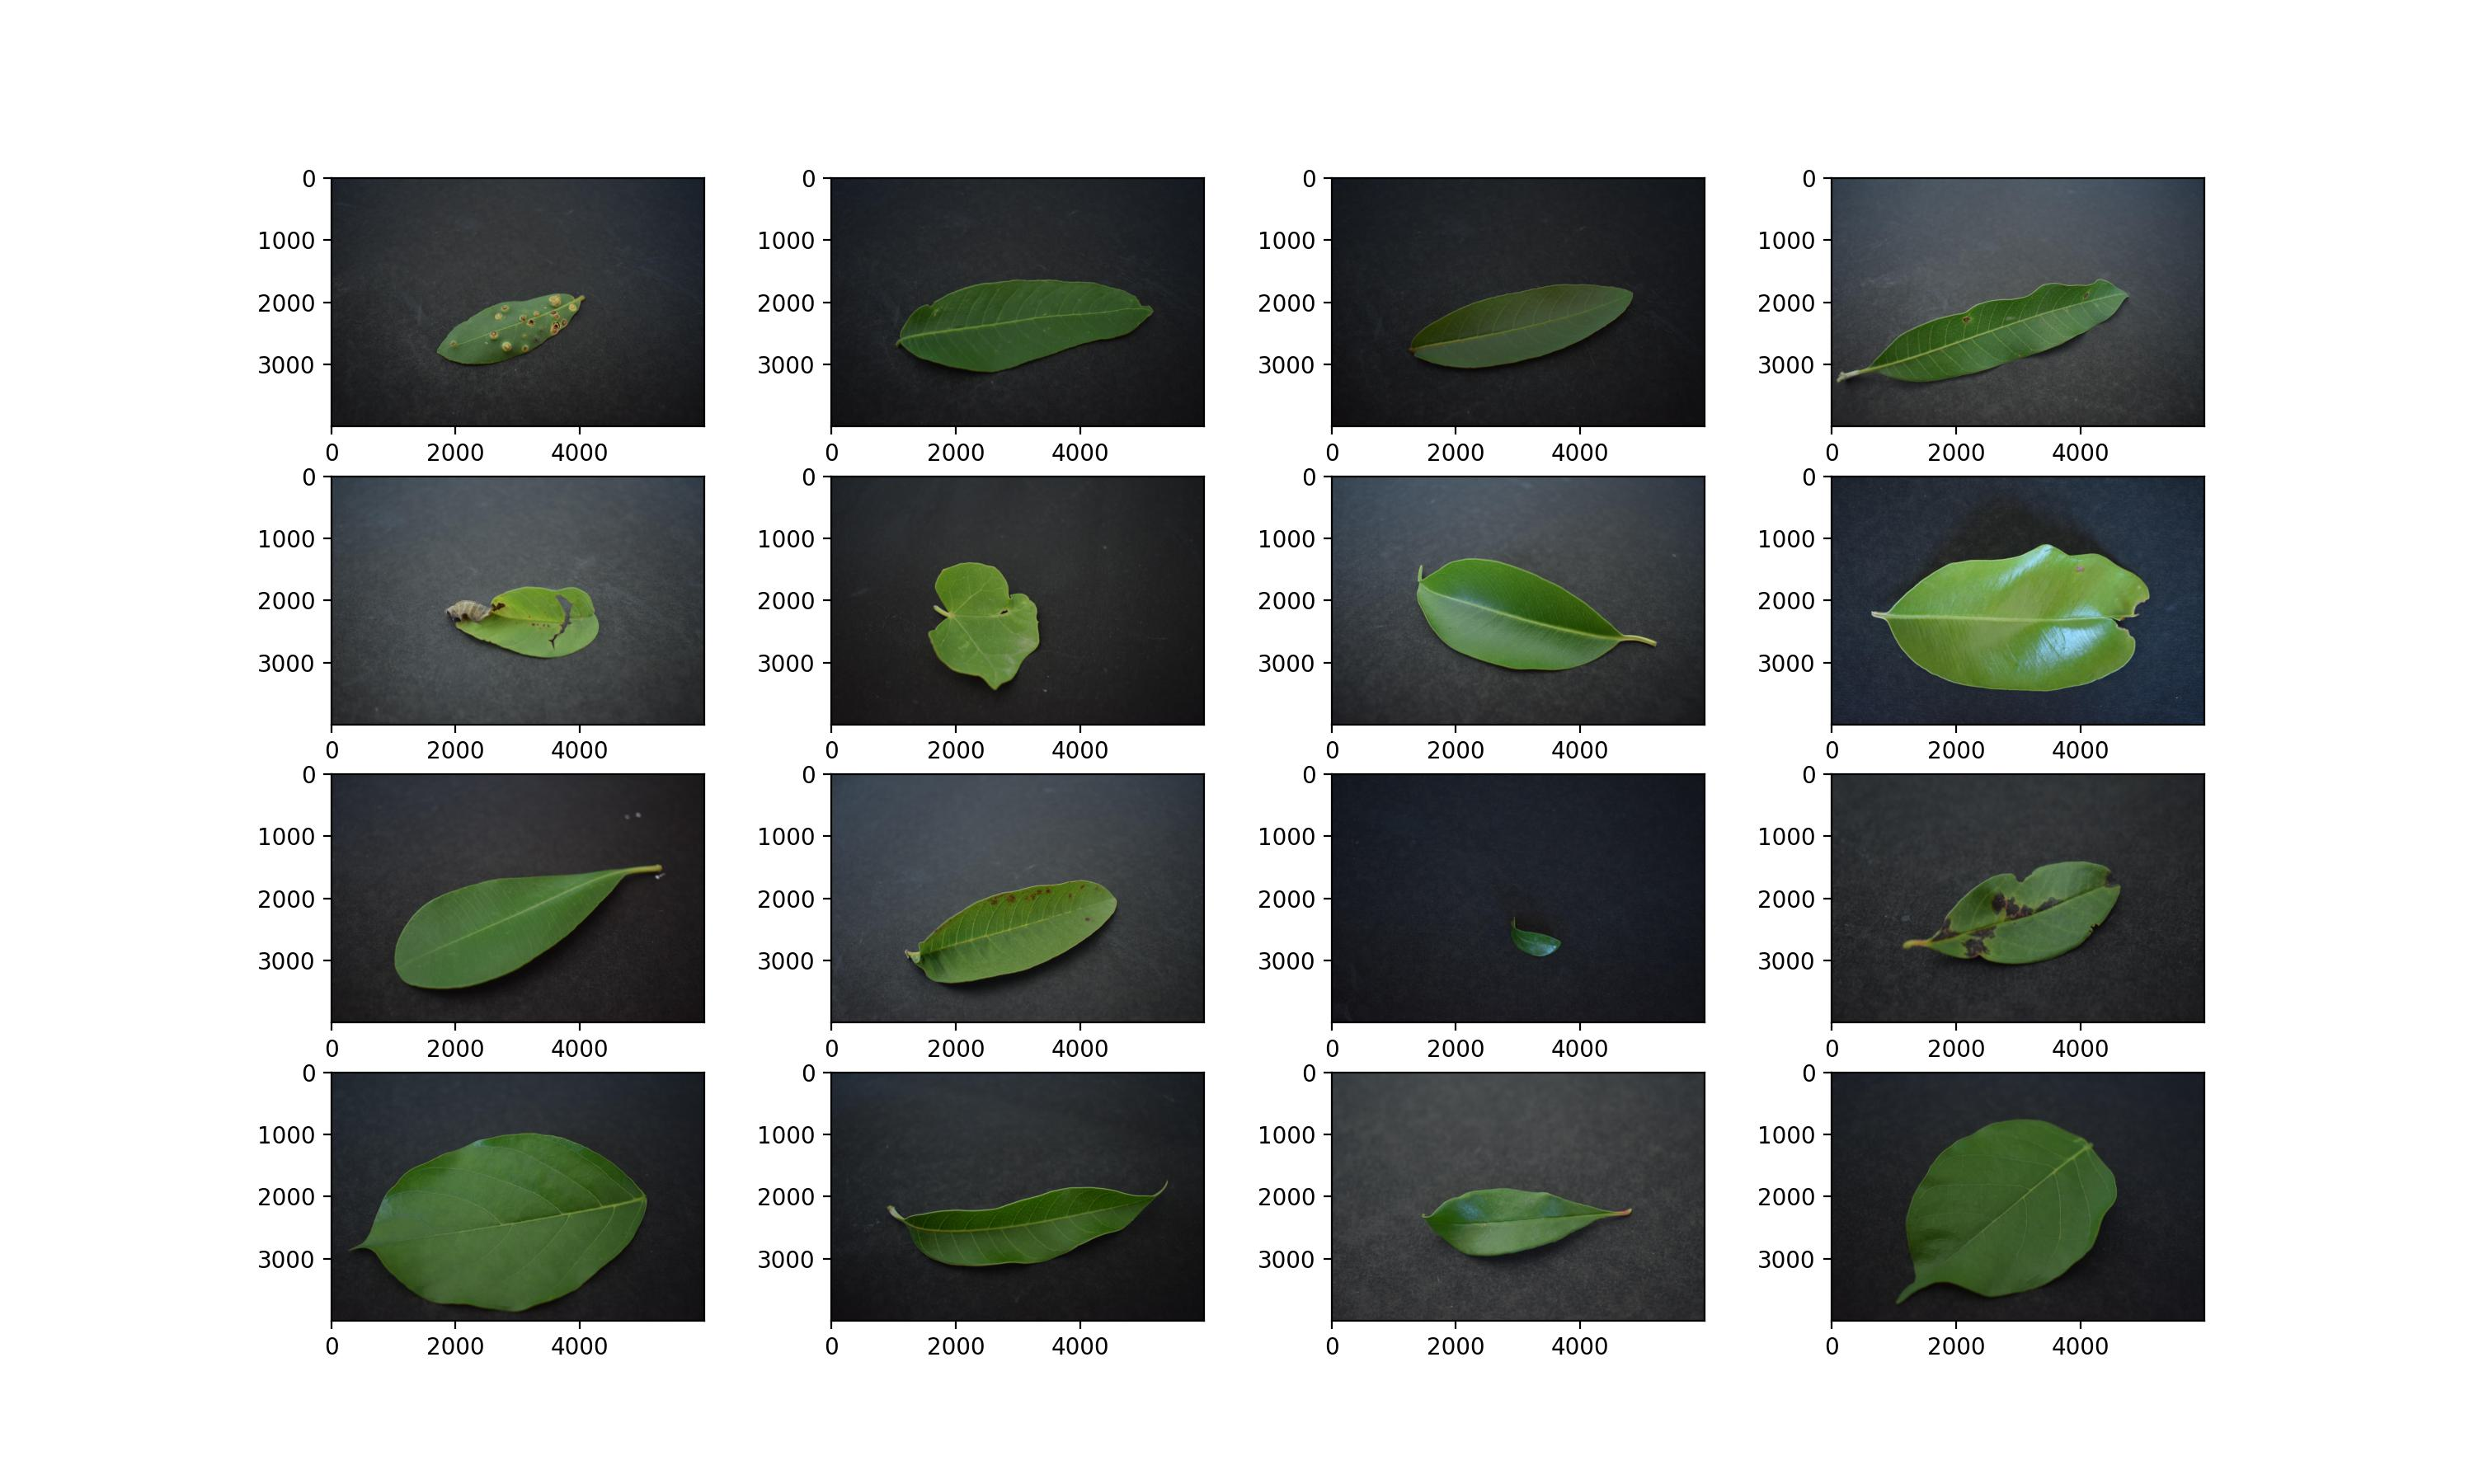
\includegraphics[width=1\textwidth]{images/sample.jpeg}
    \caption{Sample images from the training set of both healthy and diseased leaves}
    \label{fig:Fig2}
\end{figure}


\begin{table}[H]
    \begin{center}
    
    \begin{tabular}{lc}
    \multicolumn{1}{c}{\textbf{Folder}} & \multicolumn{1}{c}{\textbf{No. of images}} \\ \hline
        Train & 4,274 \\
        Validate & 110 \\
        Test & 110  \\ \hline
    \end{tabular}
    \caption{Number of images in the train, valid and test folders.} \label{tab:tab1}
    
    \end{center}
\end{table}

The data pre-processing phase starts by merging the folders 'healthy' and 'diseased' in the train, valid and test folders for every plant species available. This is, reducing 22 folders to 11 folders. Once the folders are merged and there's a single folder for each species, all images are resized to be 200x200 pixels using the \textit{imread} library. It is worth highlighting that the network requires all input images to be of the same size, as the number of nodes in the input layer is fixed, hence the resizing. \textbf{Table \ref{tab:tab2}} describes the number of images in each of the merged folders. \\

As it is clearly seen, the dataset is unbalanced, meaning that there are more images of certain categories than others. This may affect the performance of the network, as it will not learn the features of certain species as good as other ones.\\

\begin{table}[H]
    \begin{center}
    
    \begin{tabular}{lccc}
    \multicolumn{1}{c}{\textbf{Folder (labels)}} & \multicolumn{1}{c}{\textbf{Train}} & \multicolumn{1}{c}{\textbf{Valid}} & \multicolumn{1}{c}{\textbf{Test}} \\ \hline
        Alstonia Scholaris & 412 & 10 & 10\\
        Arjun & 432 & 10 & 10\\
        Basil & 244 & 10 & 10 \\
        Chinar & 203 & 10 & 10 \\
        Gauva & 398 & 10 & 10\\
        Jamun & 603 & 10 & 10\\
        Jatropha & 237 & 10 & 10\\
        Lemon & 216 & 10 & 10\\
        Mango & 414 & 10 & 10\\
        Pomegranate & 538 & 10 & 10\\
        Pongamia Pinnata & 577 & 10 & 10\\ \hline
        \textbf{Total} & \textbf{4,274} & \textbf{110} & \textbf{110} \\ \hline
    \end{tabular}
    \caption{No. of images per folder per species} \label{tab:tab2}
    
    \end{center}
\end{table}

The \textit{imread} library is also used to read the pixels of each image and transform them into RGB values to be stored as arrays. In this sense, each image is then converted into a list of 200 matrices, each one of size (200x3), with each column displaying the values of each of the three RGB channels.\\ 

The collection of matrices of the train folder is then split in two objects: the first one, containing 4,274 elements called \textit{$X_{train}$} which contains only the features of each image and the second one, \textit{$y_{train}$}, a sparse matrix of (4,274 x 11) which contains the labels of each image. The \textit{$y_{train}$} matrix is obtained through one-hot-encoding, i.e. is a [0,1] with value [1] in the column index of the corresponding label of each image and value [0] elsewhere. Finally, to simplify calculations in the network, \textit{$X_{train}$} values are normalized by a constant of 255 (the maximum of RGB pixels). This process is repeated for the valid and test folders as well.\\


\clearpage

\section{Convolutional Neural Networks} \label{Section3}

CNN as we know them nowadays can be traced back as far as the 80's, when Fukushima published the paper \emph{Neocognitron: A Self-organizing Neural Network Model for a Mechanism of Pattern Recognition Unaffected by Shift in Position} (\cite{fukushima1982neocognitron}). Further research has been done since then, but the main idea prevails: add Convolutional layers to a traditional Neural Network (NN) architecture to improve performance on computer vision tasks. The notable difference is that CNN allow us to encode image-specific features into the architecture whilst further reducing the parameters required to set up the model (\cite{o2015introduction}).\\

Simple CNN may look something like the display in \textbf{Figure \ref{fig:Fig1}}. Of course, in reality the number of convolution and hidden layers may vary depending on the task at hand, as well as their parameters. This opens up a vast and large universe of possibilities to build CNN models (no without increasing it's complexity and challenges).\\

\begin{figure}[H]
    \centering
    \includegraphics[width=0.8\textwidth]{images/Fig1.jpg}
    \caption{A simple CNN architecture, comprised of five layers (\cite{o2015introduction})}
    \label{fig:Fig1}
\end{figure}

It is worth mentioning that CNN architectures have won several different image recognition contests such as ImageNet, ICPR (Mitosis Detection in Breast Cancer), MICCAI (Medical Image Computing and Computer Assisted Interventions), IJCNN Traffic Sign Recognition Competition, among others, paving the road for further improvement as more and more real case applications are developed using these algorithms.\\

But how does this algorithm scales up with data size? Well, data size is actually where its power rests upon. These kind of algorithms are designed to be trained with thousands if not million of images, and it is imperative to do so because the more training data it has, the best performance it will yield; data quality is paramount as well, there's no much value in using high volumes of poor data. \\

The 'heavy' phase of the algorithm is then the training, because during this step that the network learns it's parameters, i.e. the weights of each node in each layer. State of the art algorithms can take a couple of days or even weeks to train, as seen in the implementation details of the VGG CNN paper (\cite{simonyan2014very}); it is worth noticing that the training times may be parallelized by using several GPUs and thus being substantially reduced.\\ 

Once learning is done, the model is saved and ready to be executed, and it can start classifying images at once. The burden of the classification depends, on how many images the algorithm may have to process at the same time, but usually this is not costly, as the CNN is not learning any more (unless configured to do so). In most cases it can be considered that a well-trained network processed more images at a given time than the ones it will process while being productive.\\

\section{Experiments and Results} \label{Section4}

Three different architectures will be trained and tested on the data. General strategy is to start with an architecture similar to the one proposed in (\cite{wu2021leaf}) and combine it with some elements from  (\cite{simonyan2014very}) for \textbf{Model 1}, then different settings will be tested for \textbf{Model 2} and \textbf{Model 3}. Training behavior of the algorithms will be validated using the validation dataset and then the risk estimate will be computed using the test set. Precision and recall scores will also be taken into account to assess the performance of the models.\\

Common ground for all models are the activation function of the output layer: the softmax function; loss will be calculated using categorical crossentropy; batch size is 32, number of epochs is 50 and early stopping is set with a patience of 5 epochs after no improvement on validation accuracy.\\

\subsection{Model 1}
Hyperparameters are displayed in \textbf{Table \ref{tab:hyper_model1}} and architecture can be seen in \textbf{Figure \ref{fig:architecture_model1}}. \\

\begin{table}[H]
    \begin{center}
    \scalebox{0.9}{
    \begin{tabular}{ll}
    \multicolumn{1}{c}{\textbf{Hyperparameters}} & \multicolumn{1}{c}{\textbf{Value}} \\ \hline
        Conv1 kernels & 16\\
        Conv2 kernels & 32\\
        Conv3 kernels & 64\\
        Kernel size & 3x3\\
        Activation & ReLU \\
        Kernel Initializer  & He uniform \\
        Padding  & Zero padding \\
        Max Pooling & 2x2 \\
        FC1 neurons & 32\\
        FC2 neurons & 16\\
        Optimizer & SGD*\\ \hline
        \multicolumn{2}{l}{*lr=0.001, momentum=0.9}\\
    \end{tabular}}
    \caption{Hyperparameters, Model 1} \label{tab:hyper_model1}
    
    \end{center}
\end{table}

\begin{figure}[H]
    \centering
    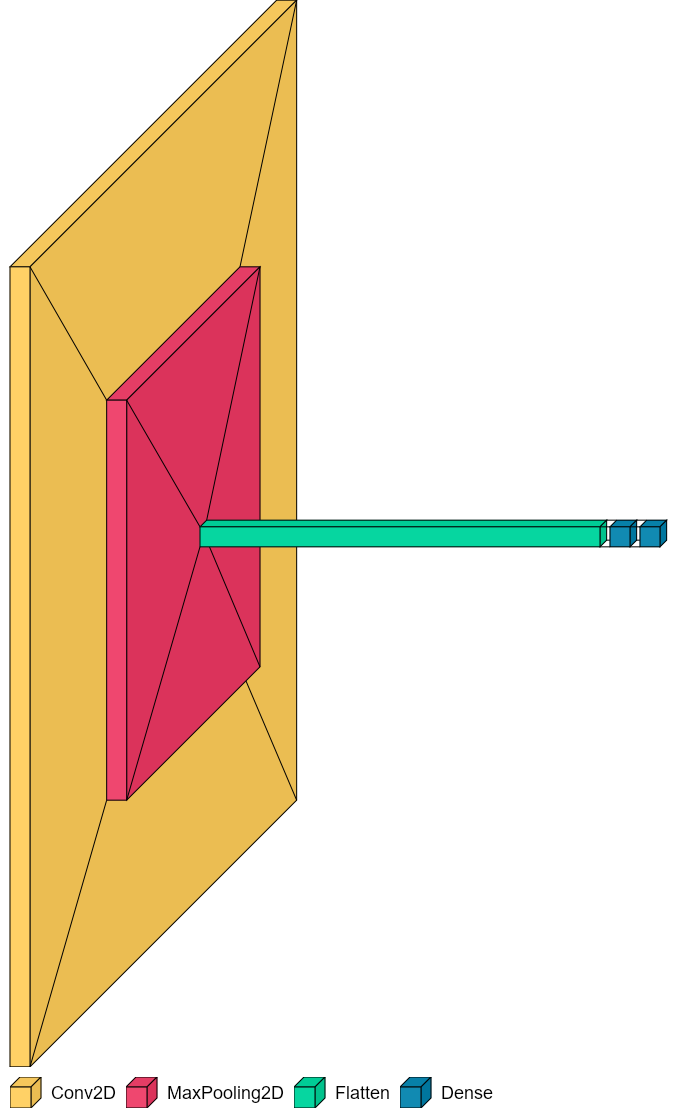
\includegraphics[width=0.75\textwidth]{images/model1_1.png}
    \caption{Architecture, Model 1}
    \label{fig:architecture_model1}
\end{figure}

Training and validation loss are plotted in \textbf{Figure \ref{fig:model1_results}}. It can be noted that the rate of learning diminishes between 10 and 15 epochs, starting to overfit the data. Around 30 epochs it is clear that the algorithm is learning noise rather than signals.
\textbf{Table \ref{tab:model1_results}} displays the average training, validation and test losses.\\


\begin{figure}[H]
    \centering
    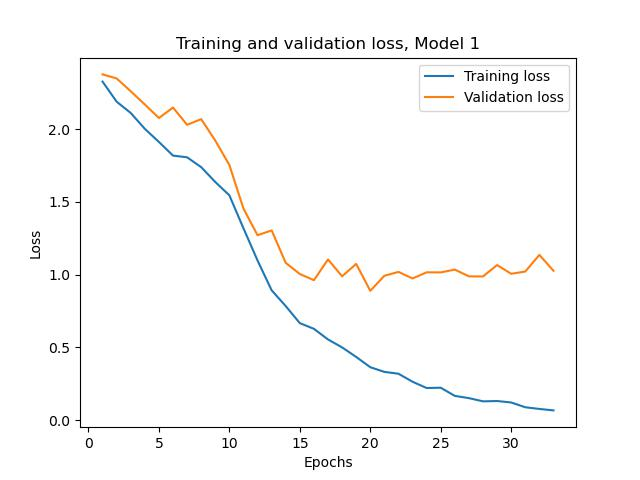
\includegraphics[width=0.75\textwidth]{images/model1_4.jpeg}
    \caption{Training and Validation loss per epochs, Model 1}
    \label{fig:model1_results}
\end{figure}


\begin{table}[H]
    \begin{center}
    
    \begin{tabular}{lr}
    \multicolumn{1}{c}{\textbf{Data}} & \multicolumn{1}{c}{\textbf{Loss}} \\ \hline
        Training & 0.8677 \\
        Validation  & 1.3812 \\
        Test  & 0.6004 \\ \hline
    \end{tabular}
    \caption{Risk estimates, Model 1} \label{tab:model1_results}
    
    \end{center}
\end{table}

\begin{table}[H]
    \begin{center}
    
    \end{center}
\end{table}


As seen in \textbf{Table \ref{tab:report_model1}}, precision and recall for \textbf{Model 1} are around 0.84 as well as its F1-score. The challenging classes for the model are Lemon, with an F1-score of 0.75 and Pongamia Pinnata, scoring 0.55 in the same metric. Besides these two categories, all the rest had a F1-score of at least 0.8.\\

\begin{table}[H]
\centering

\begin{tabular}{lrrrr}
\toprule
\multicolumn{1}{c}{\textbf{Plant type}} & \multicolumn{1}{c}{\textbf{Precision}} & \multicolumn{1}{c}{\textbf{Recall}} & \multicolumn{1}{c}{\textbf{F1-score}} & \multicolumn{1}{c}{\textbf{Support}}\\
\midrule
\textbf{Alstonia Scholaris} &       0.80 &    0.80 &      0.80 &    10.00 \\
\textbf{Arjun             } &       0.83 &    1.00 &      0.91 &    10.00 \\
\textbf{Basil             } &       0.90 &    0.90 &      0.90 &    10.00 \\
\textbf{Chinar            } &       1.00 &    0.80 &      0.89 &    10.00 \\
\textbf{Gauva             } &       0.89 &    0.80 &      0.84 &    10.00 \\
\textbf{Jamun             } &       0.71 &    1.00 &      0.83 &    10.00 \\
\textbf{Jatropha          } &       0.90 &    0.90 &      0.90 &    10.00 \\
\textbf{Lemon             } &       1.00 &    0.60 &      0.75 &    10.00 \\
\textbf{Mango             } &       0.91 &    1.00 &      0.95 &    10.00 \\
\textbf{Pomegranate       } &       1.00 &    0.80 &      0.89 &    10.00 \\
\textbf{Pongamia Pinnata  } &       0.50 &    0.60 &      0.55 &    10.00 \\ \hline
\textbf{accuracy          } &       0.84 &    0.84 &      0.84 &     0.84 \\
\textbf{macro avg         } &       0.86 &    0.84 &      0.84 &   110.00 \\
\textbf{weighted avg      } &       0.86 &    0.84 &      0.84 &   110.00 \\
\bottomrule
\end{tabular}
\caption{Classification Report, Model 1}\label{tab:report_model1}
\end{table}

\subsection{Model 2}

Innovations for \textbf{Model 2} are the following: to test a different kernel initializer, the Glorot normal is used, padding is set to valid (no padding) and a Dropout layer of 0.2 is added after each max pooling layer.  Motivation behind these minor changes is basically to test if something slightly different would achieve better results, specially with the optimizer, for which its parameters were chosen based on Keras website implementation. Hyperparameters are summarized in \textbf{Table \ref{tab:hyper_model2}} and architecture is plotted in \textbf{Figure \ref{fig:architecture_model2}}.\\

\begin{table}[H]
    \begin{center}
    \scalebox{0.9}{
    \begin{tabular}{ll}
    \multicolumn{1}{c}{\textbf{Hyperparameters}} & \multicolumn{1}{c}{\textbf{Value}} \\ \hline
        Conv1 kernels & 16\\
        Conv2 kernels & 32\\
        Conv3 kernels & 64\\
        Kernel size & 3x3\\
        Activation & ReLU \\
        Kernel Initializer  & Glorot normal \\
        Padding  & No padding \\
        Max Pooling & 2x2 \\
        Dropout (Conv) & 0.2 \\
        FC1 neurons & 32\\
        FC2 neurons & 16\\
        Optimizer & SGD*\\ \hline
        \multicolumn{2}{l}{*lr=0.001, momentum=0.9}\\
    \end{tabular}}
    \caption{Hyperparameters, Model 2} \label{tab:hyper_model2}

    \end{center}
\end{table}


\begin{figure}[H]
    \centering
    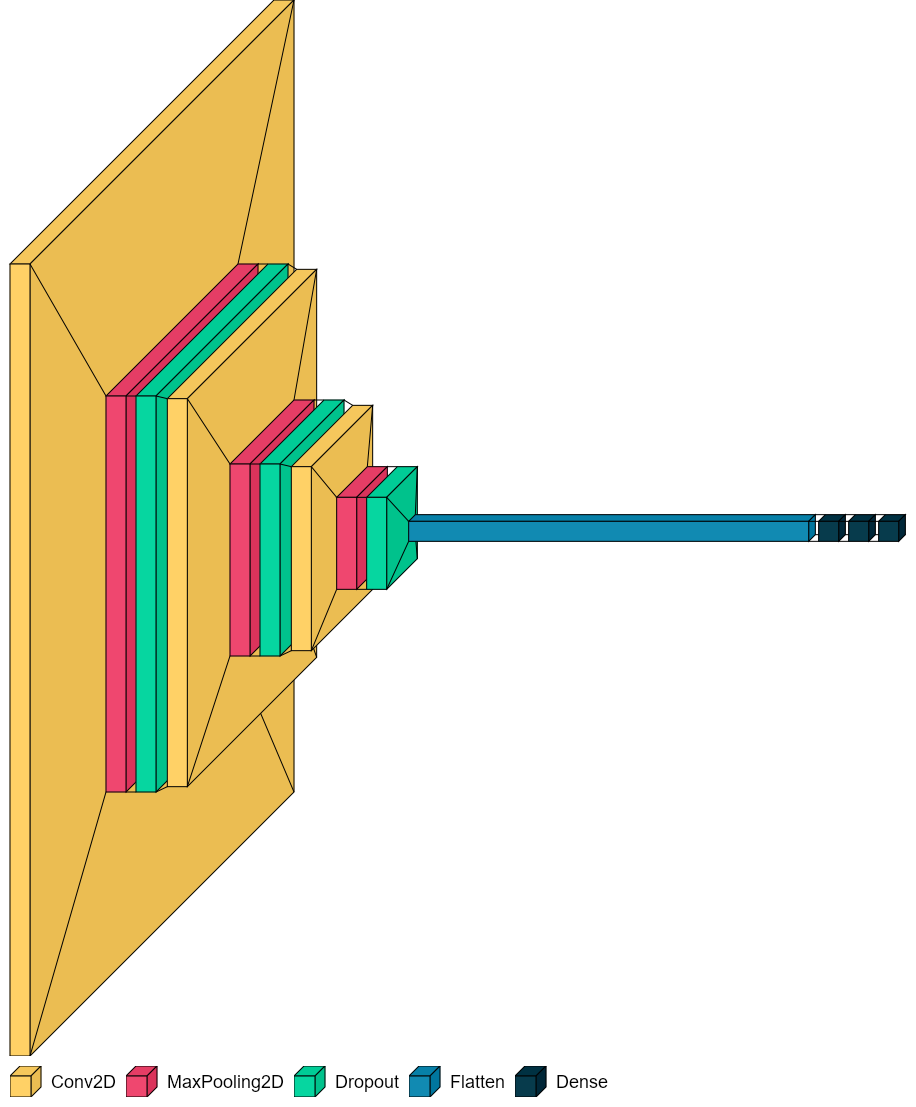
\includegraphics[width=0.75\textwidth]{images/model2_1.png}
    \caption{Architecture, Model 2}
    \label{fig:architecture_model2}
\end{figure}

Results for \textbf{Model 2} suggest an improvement in the speed of training although the risk estimates are not better if compared against \textbf{Model 1}. Another aspect to highlight is that in this case, training and validation losses are closer, whilst for the first algorithm the difference was greater. Something that is still happening is that the test set has a lower loss than the validation estimates.\\

\begin{figure}[H]
    \centering
    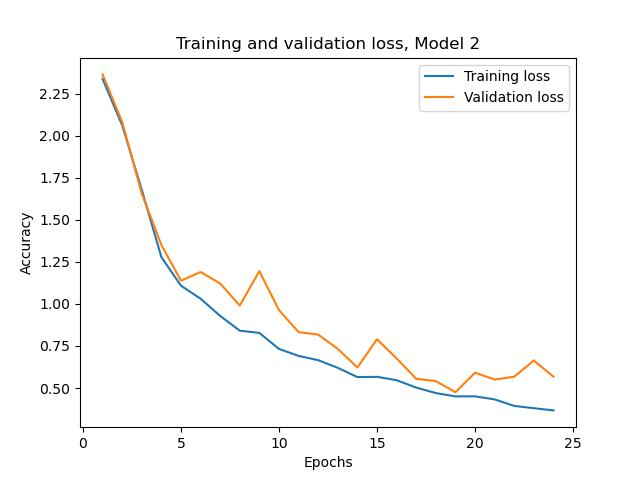
\includegraphics[width=0.75\textwidth]{images/model2_4.jpeg}
    \caption{Training and Validation loss per epochs, Model 2}
    \label{fig:model2_results}
\end{figure}

\begin{table}[H]
    \begin{center}
    
    \begin{tabular}{lc}
    \multicolumn{1}{c}{\textbf{Data}} & \multicolumn{1}{c}{\textbf{Loss}} \\ \hline
        Training & 1.2427 \\
        Validation  & 1.4152 \\
        Test  & 0.9652 \\ \hline
    \end{tabular}
    \caption{Risk estimates, Model 2} \label{tab:model2_results}
    
    \end{center}
\end{table}

Results for classification performance of \textbf{Model 2} are shown in \textbf{Table \ref{tab:report_model2}}.  Precision and recall for  are around 0.6, with precision having a slightly better score than recall, meaning a higher proportion of true positives against false positives, but also a relatively high incidence of false negatives. This time, the categories most missmatched were Chinar, Gauva, Jatropha, Lemon and Pongamia Pinnata, as for the F1-score. Only one category, Mango, had a F1-score of 0.9.\\

\begin{table}[H]
\centering

\begin{tabular}{lrrrr}
\toprule
\multicolumn{1}{c}{\textbf{Plant type}} & \multicolumn{1}{c}{\textbf{Precision}} & \multicolumn{1}{c}{\textbf{Recall}} & \multicolumn{1}{c}{\textbf{F1-score}} & \multicolumn{1}{c}{\textbf{Support}}\\
\midrule
\textbf{Alstonia Scholaris} &       0.75 &    0.60 &      0.67 &    10.00 \\
\textbf{Arjun             } &       0.64 &    0.70 &      0.67 &    10.00 \\
\textbf{Basil             } &       0.53 &    0.90 &      0.67 &    10.00 \\
\textbf{Chinar            } &       1.00 &    0.20 &      0.33 &    10.00 \\
\textbf{Gauva             } &       0.67 &    0.40 &      0.50 &    10.00 \\
\textbf{Jamun             } &       0.56 &    1.00 &      0.71 &    10.00 \\
\textbf{Jatropha          } &       0.80 &    0.40 &      0.53 &    10.00 \\
\textbf{Lemon             } &       0.75 &    0.30 &      0.43 &    10.00 \\
\textbf{Mango             } &       0.90 &    0.90 &      0.90 &    10.00 \\
\textbf{Pomegranate       } &       0.73 &    0.80 &      0.76 &    10.00 \\
\textbf{Pongamia Pinnata  } &       0.33 &    0.60 &      0.43 &    10.00 \\ \hline
\textbf{accuracy          } &       0.62 &    0.62 &      0.62 &     0.62 \\
\textbf{macro avg         } &       0.70 &    0.62 &      0.60 &   110.00 \\
\textbf{weighted avg      } &       0.70 &    0.62 &      0.60 &   110.00 \\ 
\bottomrule
\end{tabular}
\caption{Classification Report, Model 2}\label{tab:report_model2}
\end{table}


\subsection{Model 3}

Given the results registered in \textbf{Model 2} against \textbf{Model 1}, \textbf{Model 3} will not have any Dropout layer, as it may had accelerated the training stage too much. This time, innovations are: optimizer is switched to Adam instead of SGD, padding is same (zero-padding) as in \textbf{Model 1} and a fourth convolutional layer is added before the fully connected layer.

\begin{table}[H]
    \begin{center}
    \scalebox{0.9}{
    \begin{tabular}{ll}
    \multicolumn{1}{c}{\textbf{Hyperparameters}} & \multicolumn{1}{c}{\textbf{Value}} \\ \hline
        Conv1 kernels & 16\\
        Conv2 kernels & 32\\
        Conv3 kernels & 64\\
        Conv3 kernels & 128\\
        Kernel size & 3x3\\
        Activation & ReLU \\
        Kernel Initializer  & Glorot normal \\
        Padding  & Zero padding \\
        Max Pooling & 2x2 \\
        FC1 neurons & 32\\
        FC2 neurons & 16\\
        Optimizer & Adam*\\ \hline
       \multicolumn{2}{l}{ *lr=0.001, $\textbeta1=0.9$, $\textbeta2=0.999$, $\textepsilon=1x10^{-7}$ }
    \end{tabular}}
    \caption{Hyperparameters, Model 3} \label{tab:hyper_model3}

    \end{center}
\end{table}

\begin{figure}[H]
    \centering
    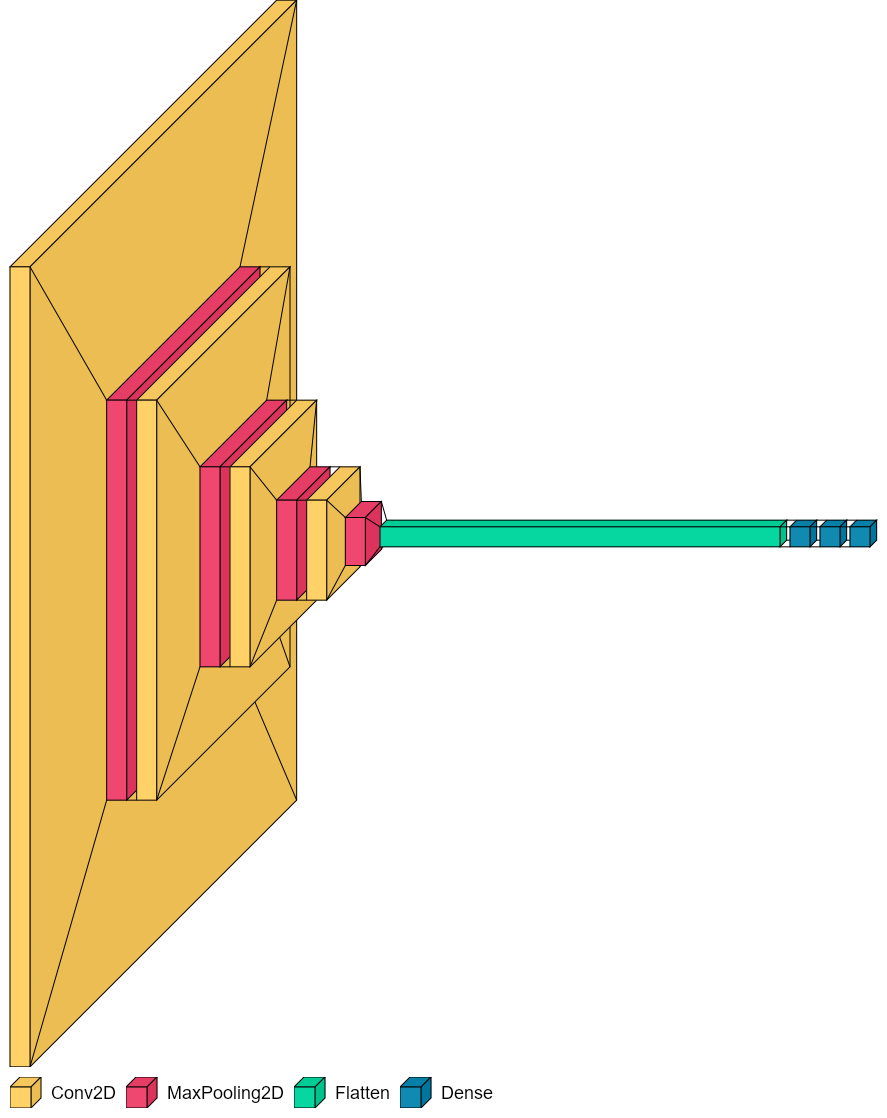
\includegraphics[width=0.75\textwidth]{images/model3_1.png}
    \caption{Architecture, Model 3}
    \label{fig:architecture_model3}
\end{figure}

Results regarding training speed remain more or less the same as in \textbf{Model 2}, with the difference that this time the training, validation and test loss are the lowest amongst the three algorithms tested. Same puzzling result happening in \textbf{Model 3}, test loss is lower than training and validation losses, while it should be higher.

\begin{figure}[H]
    \centering
    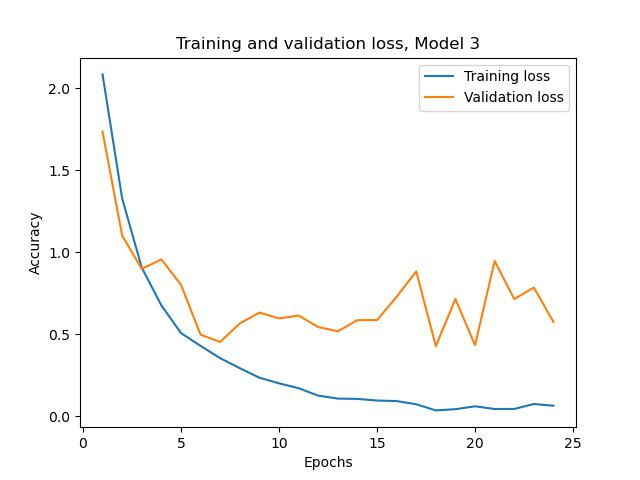
\includegraphics[width=0.75\textwidth]{images/model3_4.jpeg}
    \caption{Training and Validation loss per epochs, Model 3}
    \label{fig:model3_val}
\end{figure}

\begin{table}[H]
    \begin{center}
    
    \begin{tabular}{lr}
    \multicolumn{1}{c}{\textbf{Data}} & \multicolumn{1}{c}{\textbf{Loss}} \\ \hline
        Training & 0.3991 \\
        Validation  & 0.5962 \\
        Test  & 0.3321 \\ \hline
    \end{tabular}
    \caption{Risk estimates, Model 3} \label{tab:model3_results}
    
    \end{center}
\end{table}

Regarding the classification performance, it is the higher amongst the three models. with values around 0.93. The worst-scoring category was Gauva, with a F1-score of 0.86, a score that would have been on the higher tier for \textbf{Model 1}. Several other categories reached a F1-score of 0.9 or higher, and precision and recall did not registered huge differences between each other.

\begin{table}[H]
\centering
\begin{tabular}{lrrrr}
\toprule
\multicolumn{1}{c}{\textbf{Plant type}} & \multicolumn{1}{c}{\textbf{Precision}} & \multicolumn{1}{c}{\textbf{Recall}} & \multicolumn{1}{c}{\textbf{F1-score}} & \multicolumn{1}{c}{\textbf{Support}}\\
\midrule
\textbf{Alstonia Scholaris} &       0.83 &    1.00 &      0.91 &    10.00 \\
\textbf{Arjun             } &       0.91 &    1.00 &      0.95 &    10.00 \\
\textbf{Basil             } &       0.83 &    1.00 &      0.91 &    10.00 \\
\textbf{Chinar            } &       1.00 &    0.90 &      0.95 &    10.00 \\
\textbf{Gauva             } &       0.82 &    0.90 &      0.86 &    10.00 \\
\textbf{Jamun             } &       0.91 &    1.00 &      0.95 &    10.00 \\
\textbf{Jatropha          } &       1.00 &    0.80 &      0.89 &    10.00 \\
\textbf{Lemon             } &       1.00 &    0.90 &      0.95 &    10.00 \\
\textbf{Mango             } &       1.00 &    1.00 &      1.00 &    10.00 \\
\textbf{Pomegranate       } &       1.00 &    0.90 &      0.95 &    10.00 \\
\textbf{Pongamia Pinnata  } &       1.00 &    0.80 &      0.89 &    10.00 \\ \hline
\textbf{accuracy          } &       0.93 &    0.93 &      0.93 &     0.93 \\
\textbf{macro avg         } &       0.94 &    0.93 &      0.93 &   110.00 \\
\textbf{weighted avg      } &       0.94 &    0.93 &      0.93 &   110.00 \\
\bottomrule
\end{tabular}
\caption{Classification Report, Model 3}\label{report_model1}
\end{table}

\clearpage

\begin{center}
    \section{Conclusions}
    \label{Results}
\end{center}

With the objective of testing  an algorithm that could classify plant leaves accurately and could be capable to process thousands or even millions of inputs, a Convolutional Neural Network algorithm was proposed, and three different variants were tested. The core ideas behind the architecture come from the literature and the plethora of resources available in the internet, while the parameter tunning strategy and fine details are inputs from the author.\\

As seen in the code and by the nature of Neural Networks, scaling these algorithms is as easy as saving more pictures of leaves in the corresponding folders for training, validation, and testing. The algorithm will run independently and does not need to be 'tweaked', unless a very big amount of data should be processed, for which case a parallelization method should be implemented, maximizing computing capacity available through a GPU.\\

Of course, this exercise has opened several different paths for hypothesis and further testing. Improvements could come from adjustments to hyperparameters as obvious as the number of epochs or patience factor, or from slight changes in the learning rate of the optimizers. A first improvement should come from the input data, having a balanced dataset in all categories would ease the interpretability of results and would guarantee a 'fair' learning phase for the algorithm. Either way, room for imrpovement is large, and a sound strategy could be to create a network that learns slower, but steadier, starting from \textbf{Model 3}, which registered the best results of all tested algorithms.\\

Factors that seemed to have positive results are: zero padding, Adam optimizer and no dropout layer. It is not clear if kernel initializer should be He uniform or Glorot normal. Also, four convolutional layers seemed to improve results when compared to three convolutional layers architecture. A puzzling pattern seen during all testing was test loss scores lower than training and validation losses, this could be explained by the fact that very few images are available for testing, and a more robust test dataset should provide a more accurate estimation of the risk. Finally, a table summarizing the key metrics to assess model performance is shown \textbf{Table \ref{tab:final_results}}:\\

\begin{table}[H]
    \begin{center}
    
    \begin{tabular}{lrrr}
    \multicolumn{1}{c}{\textbf{Metric}} & \multicolumn{1}{c}{\textbf{Model 1}} & 
    \multicolumn{1}{c}{\textbf{Model 2}} & \multicolumn{1}{c}{\textbf{Model 3}}\\ \hline
        Training loss & 0.8677 & 1.2427& 0.3991 \\
        Validation loss  & 1.3812 & 1.4152 & 0.5962\\
        Test loss  & 0.6004 & 0.9652 & 0.3321\\ \hline
        w.avg. Precision & 0.84 & 0.70 & 0.94 \\
        w.avg. Recall & 0.84 & 0.62 & 0.93 \\
        w.avg. F1-score & 0.86 & 0.60 & 0.93\\ \hline
    \end{tabular}
    \caption{Metrics per model} \label{tab:final_results}
    
    \end{center}
\end{table}


\clearpage

\begin{center}
    \section*{Bibliography}
\end{center}

\printbibliography

\end{document}




